\section{System Architecture}
\label{sa}
\todo{Figures}
To achieve the goal of high maintainability a back plane architecture was chosen \todo{reference back plane}. The choice of back plane is also defended as a way to eliminate wires and connectors between different pcbs, as wires can fall out during transport, and glue is not an alternative as it should be easy to change a module. The backplane provides a good electrical and mechanical connection as well as some additional features. \todo{Revise sentence, move someplace else?}

The signal source needs to be a long distance away from the coil rig due to safety reasons, and the power amplifier needs to be as close to the coil rig as possible to keep ohmic losses in the resonant circuit as low as possible. The Interrupter and power limiter has low voltage feedback signals X8 and X9 as inputs. Because of the nature of a tesla coil, there is a lot of electromagnetic interference (EMI) present such that low voltage signals needs to be sent through a channel that is robust against electromagnetical noise. Thus the system is partitioned such that the signal source and pulse shaper TK100 is placed together, and the rest of the system placed together in a shielded enclosure TK500. The signal from the pulse shaper X2 should then be sent through a robust channel. Optical plastic fibre is chosen described in \cref{optical}. X8 and X9 are then short and inside a shielded enclosure, and no other protection from EMI is required.

Inside TK500 we have both high power and low power signals. These should be separated such that the high power signals does not provide interference for the low power signals. And so that the electronics with low power signals can be designed with lower voltage and power requirements. This is solved by creating a signal back plane TK510 and a power back plane TK530, connected via an galvanic isolation TK520.

In addition some user interface is needed on the driver TK500 This is partitioned into a sub system called TK540.

%Bus on back plane, pros: can insert card anywhere cons: risk of inserting two of one card.

 
\subsection{Card inserted bus}
When partitioning the system into several modules physically spread over multiple pcbs there is a risk of one module not being connected to the system, either because of issues with transportation, or by human error. To mitigate this risk, detection of wich cards is inserted into the back plane is implemented. This is done by a bus \todo{Specify wich kind of bus and reference.} \todo{Draw bus architecture}
The bus consists of one wire named Kort\_innsatt, pulled high by a $10k\Omega$ resistor, \cref{fig:ki_bi} shows how each card slot interfaces to the card inserted bus, KI is connected to the card slot and Kort\_innsatt is the bus. When no card is inserted into the slot KI is left floating and the gate of the nmos is pulled high by R53001 and the nmos goes into the triode region and pulls the bus low. When a card is inserted it pulls KI low. And the nmos goes into cut-off.\todo{More figures}

\begin{figure}[h]
    \centering
    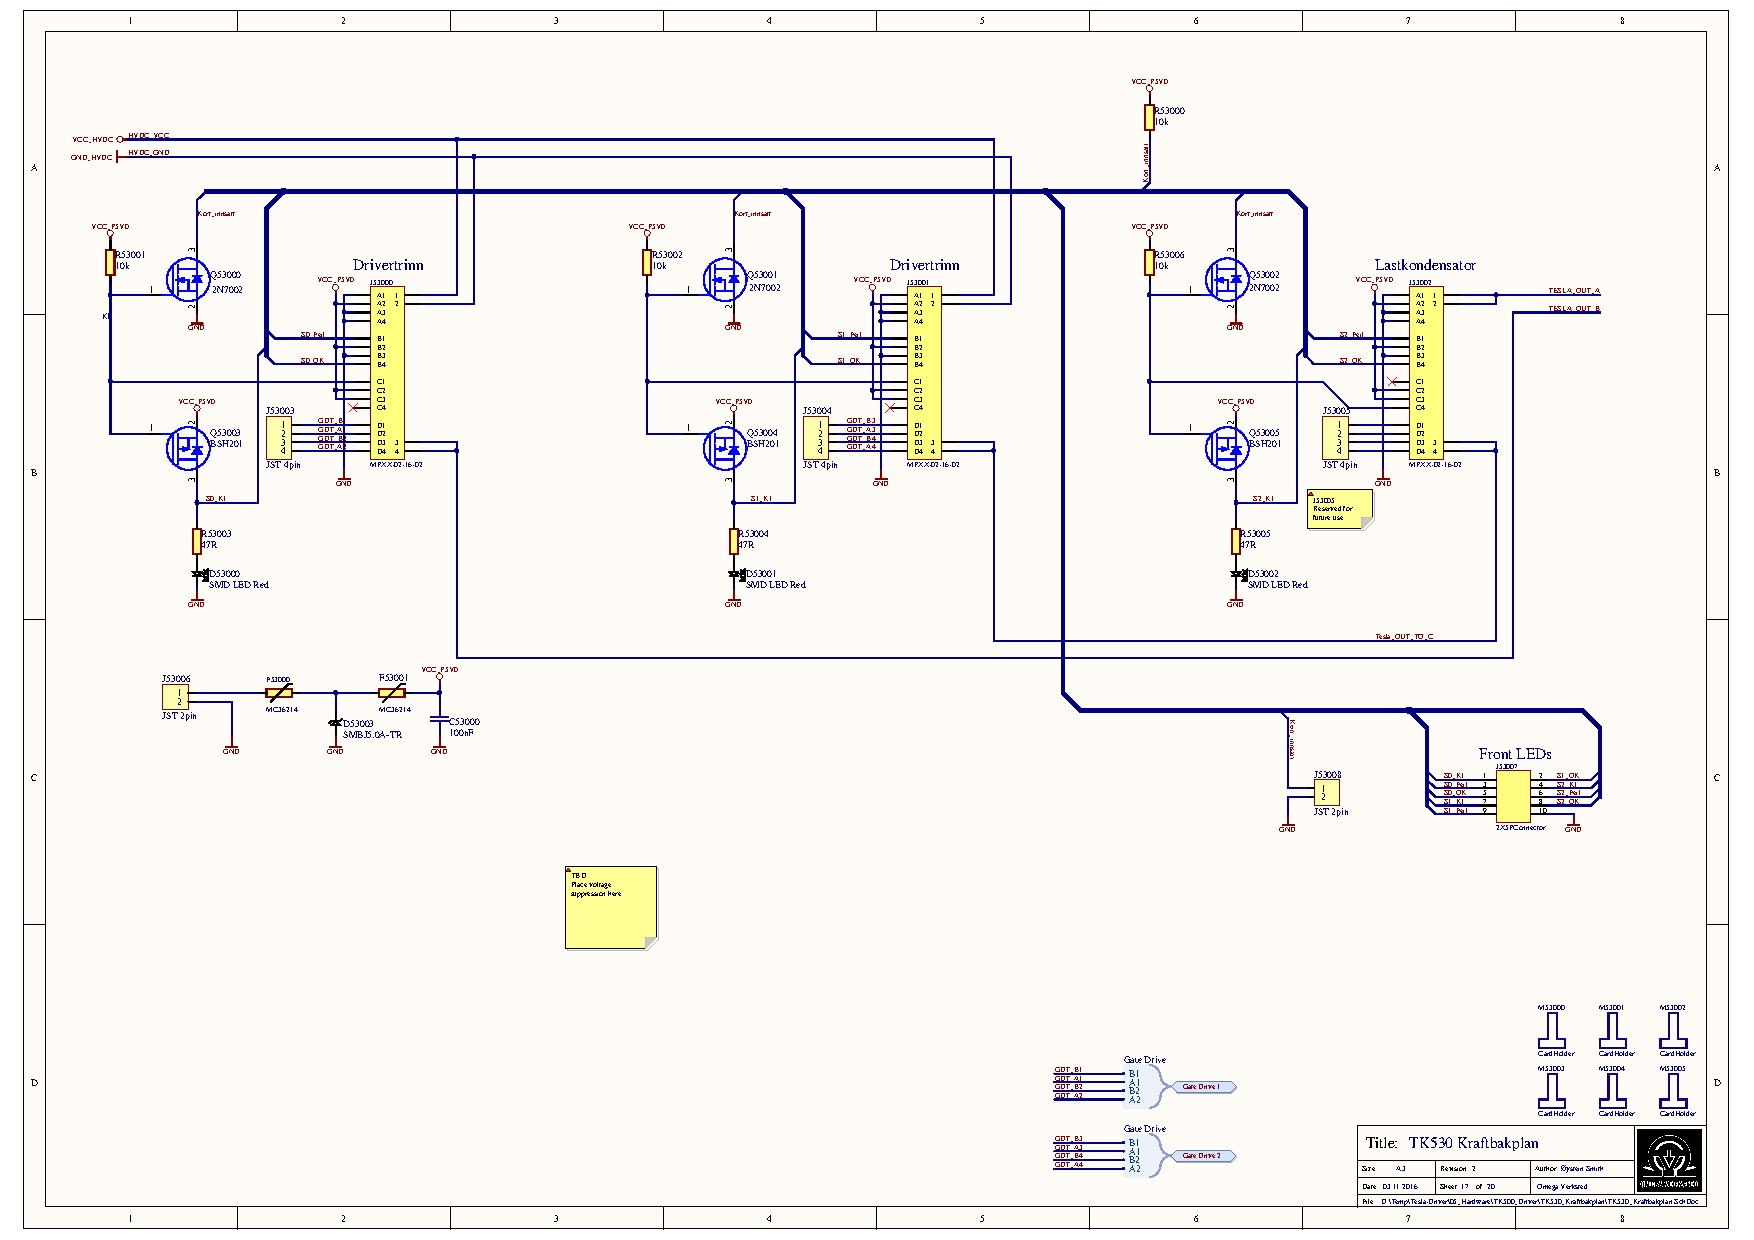
\includegraphics[trim={1cm 15cm 25.5cm 3cm},clip,width=8cm]{img/TK530_Kraftbakplan.pdf}
    \caption{Bus interface (detail from schematic of TK530 Kraftbakplan)}
    \label{fig:ki_bi}
\end{figure}
\todo{add switch to figure}

\subsection{Optical channel}
\label{optical}

\subsection{Bus}
\label{bus}

\subsection{Individual module signals}